\documentclass{article}

\usepackage[main=english,vietnamese]{babel}
\usepackage[T1]{fontenc}
\usepackage[utf8]{inputenc}
\usepackage[sexy]{evan}
\usepackage{matchsticks}
\usepackage{wrapfig}
\usepackage{listings}

\newtheorem{hint}{Hint}

\title{Derivative II}
\author{Nghia Doan}
\date{\today}

\begin{document}

\maketitle

\begin{problem*}[1a]
    We restrict the function $\sec(x)$ on $\left[ 0, \frac{\pi}{2} \right) \cup \left[ \pi, \frac{3\pi}{2} \right)$ to get an one-to-one function.
    We call it $f(x).$ We define the inverse of this function be $f^{-1}(x).$

    Find the domain and range of $f^{-1}.$
\end{problem*}

\begin{center}
    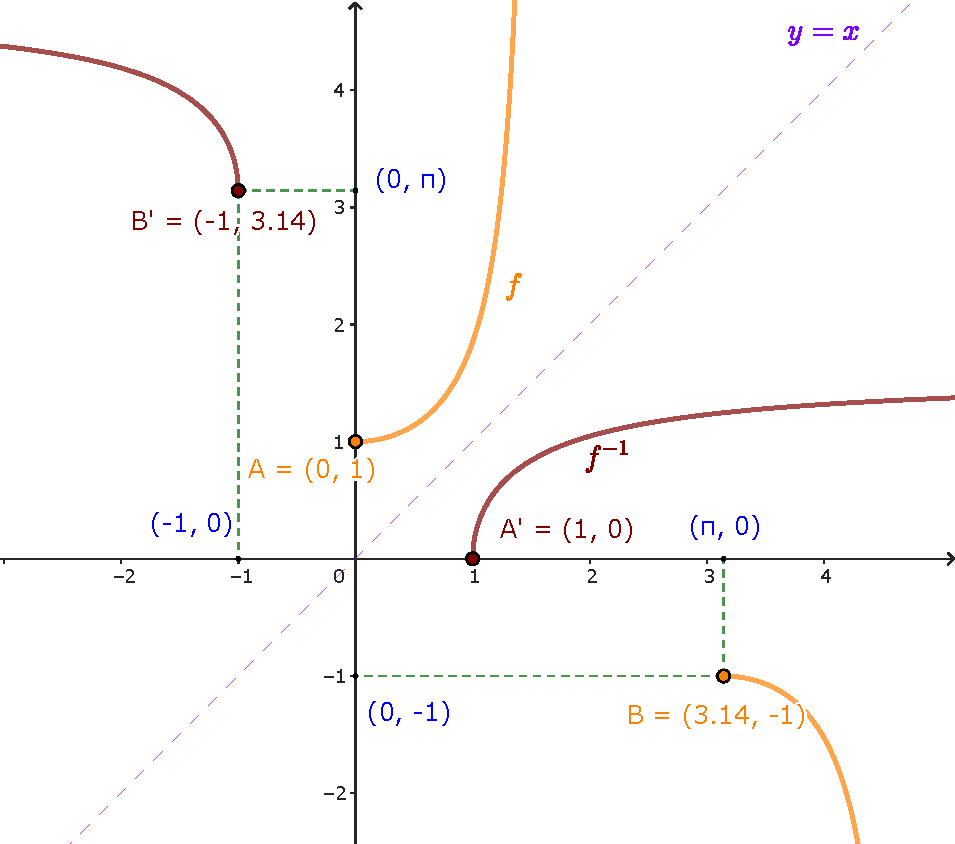
\includegraphics[width=12cm]{./svg/pdf/derivative-2-1a.pdf}
\end{center}

\begin{soln}
    First,
    \[
        f(x) = \sec(x) = \frac{1}{\cos(x)}.
    \]

    Since $\cos(x)$ strictly decreases from $1$ to $0$ on $\left[ 0, \frac{\pi}{2} \right),$ 
    thus $f(x)$ strictly increases from $1$ to $+\infty$ on this interval.
    Similarly $\cos(x)$ strictly increases from $-1$ to $0$ on $\left[ \pi, \frac{3\pi}{2} \right),$ 
    thus $f(x)$ strictly decreases from $-1$ to $-\infty$ on this interval.
    Thus, $f(x)$ is a one-to-one function.

    Since $f$ is a one-on-one function, the domain of $f^{-1}$ is the range of $f,$ and vice versa,
    \[
        D_{f^{-1}} = R_f = \left( -\infty, -1 \right] \cup \left[ 1, +\infty \right),\
        R_{f^{-1}} = D_f = \left[ 0, \frac{\pi}{2} \right) \cup \left[ \pi, \frac{3\pi}{2} \right).
    \]
\end{soln}

\begin{problem*}[1b]
    Compute $f^{-1}(sec(5))$ and $sec(f^{-1}(5)).$
\end{problem*}

\begin{center}
    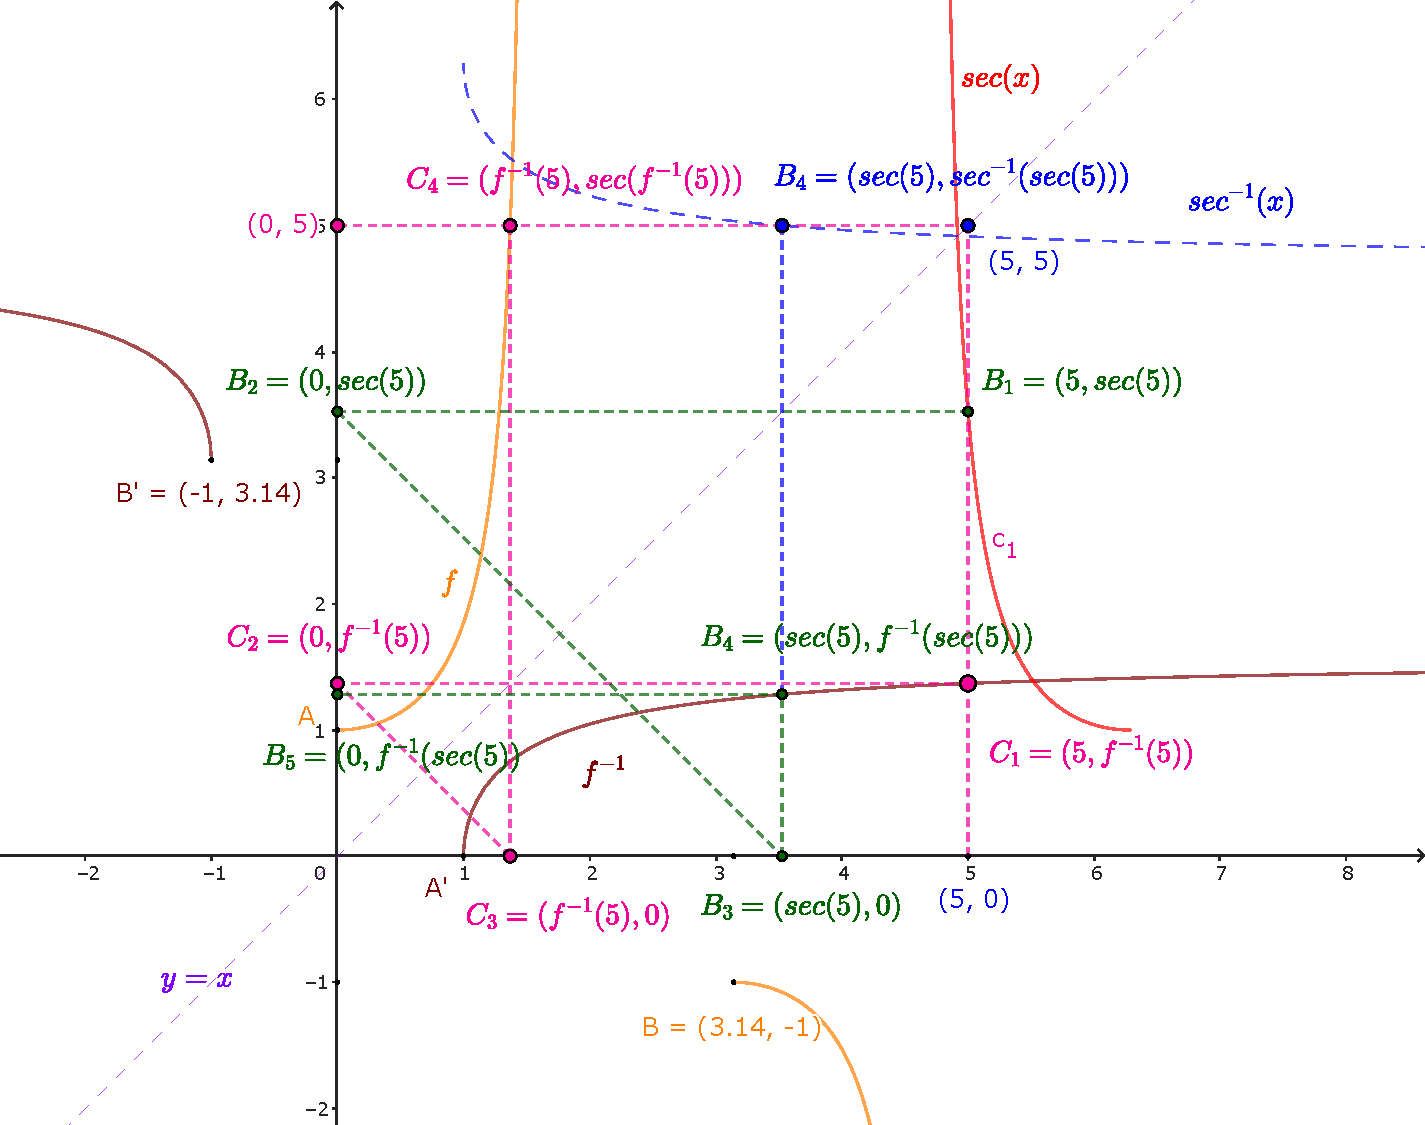
\includegraphics[width=15cm]{./svg/pdf/derivative-2-1b.pdf}
\end{center}

\begin{soln}
    First,
    \[
        \begin{aligned}
            &\sec(5) \approx 3.525 \Rightarrow f^{-1}(\sec(5)) \approx 1.28 \quad (B_4\ \text{green})\\
            &f^{-1}(5) \approx 1.37 \Rightarrow \sec(f^{-1}(5)) = \sec(1.37) \approx 5.01 \quad (C_4\ \text{purple})\\
        \end{aligned}
    \]

    \textit{For $f^{-1}(\sec(5)),$} follow the chain of points:
    \[
        (5,0) \rightarrow B_1 = (5, \sec(5)) \rightarrow B_2 = (0, \sec(5)) \rightarrow B_3 = (\sec(5), 0)
        \rightarrow B_4 =  (\sec(5), f^{-1}(\sec(5))),
    \]
    which does not lead to $f^{-1}(\sec(5))=5.$
    The reason is that $\frac{3\pi}{2} < 5,$ outside of $D_f,$ thus for the value $\sec(5) = 3.525$ the function $f^{-1}$ returns $1.28$ instead.
    Consider $\sec^{-1}$ ($B_4$ blue) for that value, it shall returns $\sec^{-1}(\sec(5)) = 5.$

    \textit{For $\sec(f^{-1}(5)),$}  follow the chain of points:
    \[
        (5,0) \rightarrow C_1 = (5, f^{-1}(5)) \rightarrow C_2 = (0, f^{-1}(5)) \rightarrow C_3 = (f^{-1}(5), 0)
        \rightarrow C_4 =  (f^{-1}(5), \sec(f^{-1}(5), 0)) \rightarrow (5,5)
    \]
\end{soln}

\newpage

\begin{problem*}[1c]
    Sketch the graph of $\sec \circ f^{-1}.$ Make sure to label your axes and that you have the correct domain.
\end{problem*}

\begin{center}
    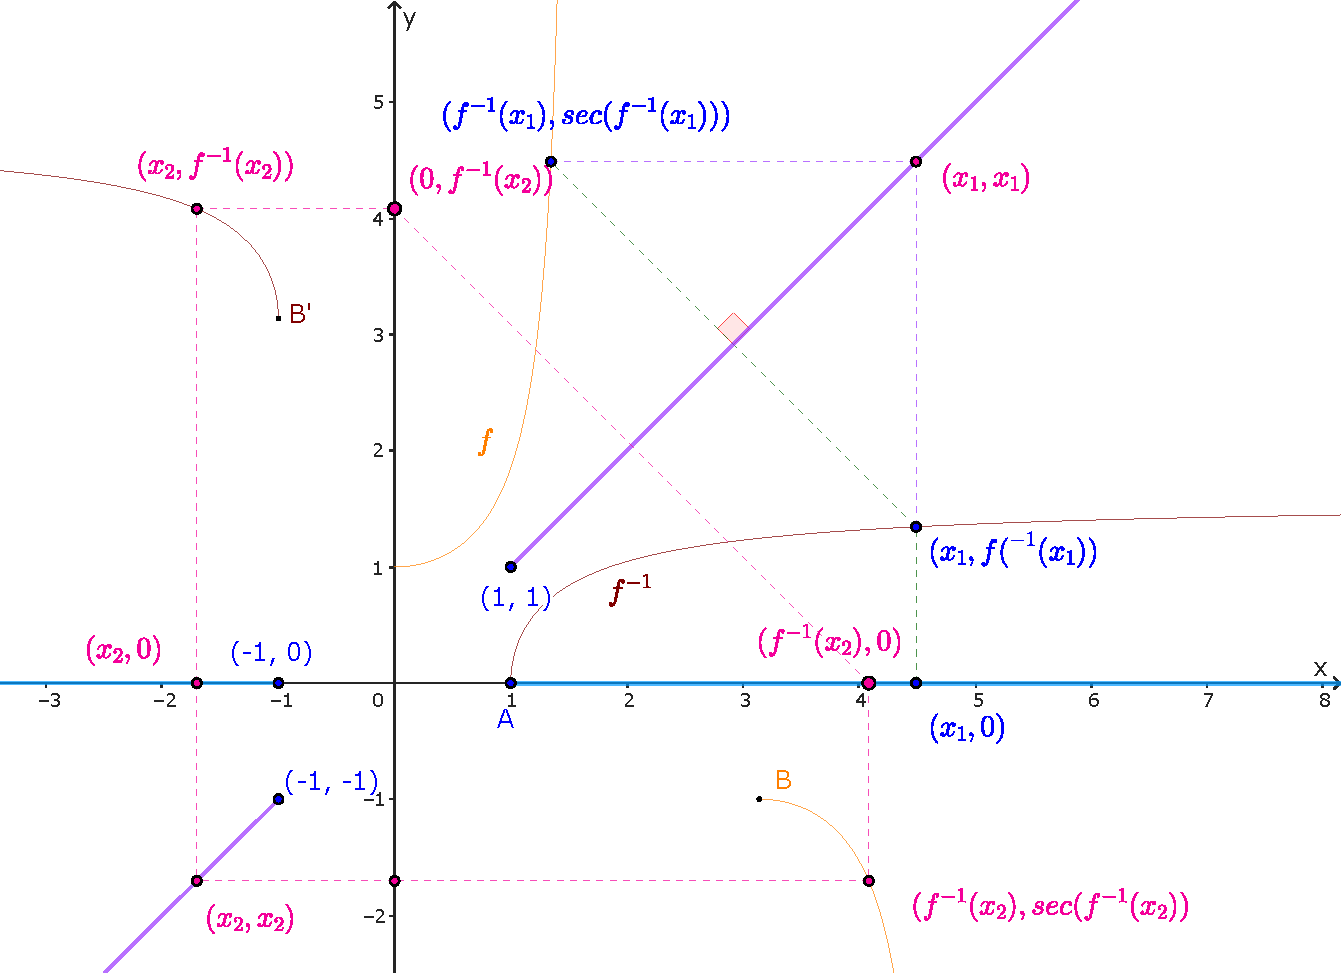
\includegraphics[width=16cm]{./svg/pdf/derivative-2-1c.pdf}
\end{center}

\begin{soln}
    Note that the graph of $\sec \circ f^{-1}$ consists of two rays
    \[
        (sec \circ f^{-1})(x) = 
        \begin{cases}
            &r_1:\ \left( -\infty, -1 \right] \rightarrow \RR,\ r_1(x) = x\\
            &r_2:\ \left[ +1, +\infty \right) \rightarrow \RR,\ r_2(x) = x\\
        \end{cases}
    \]
\end{soln}

\newpage

\begin{problem*}[1d]
    Sketch the graph of $f^{-1} \circ \sec.$ Make sure to label your axes and that you have the correct domain.
\end{problem*}

\begin{center}
    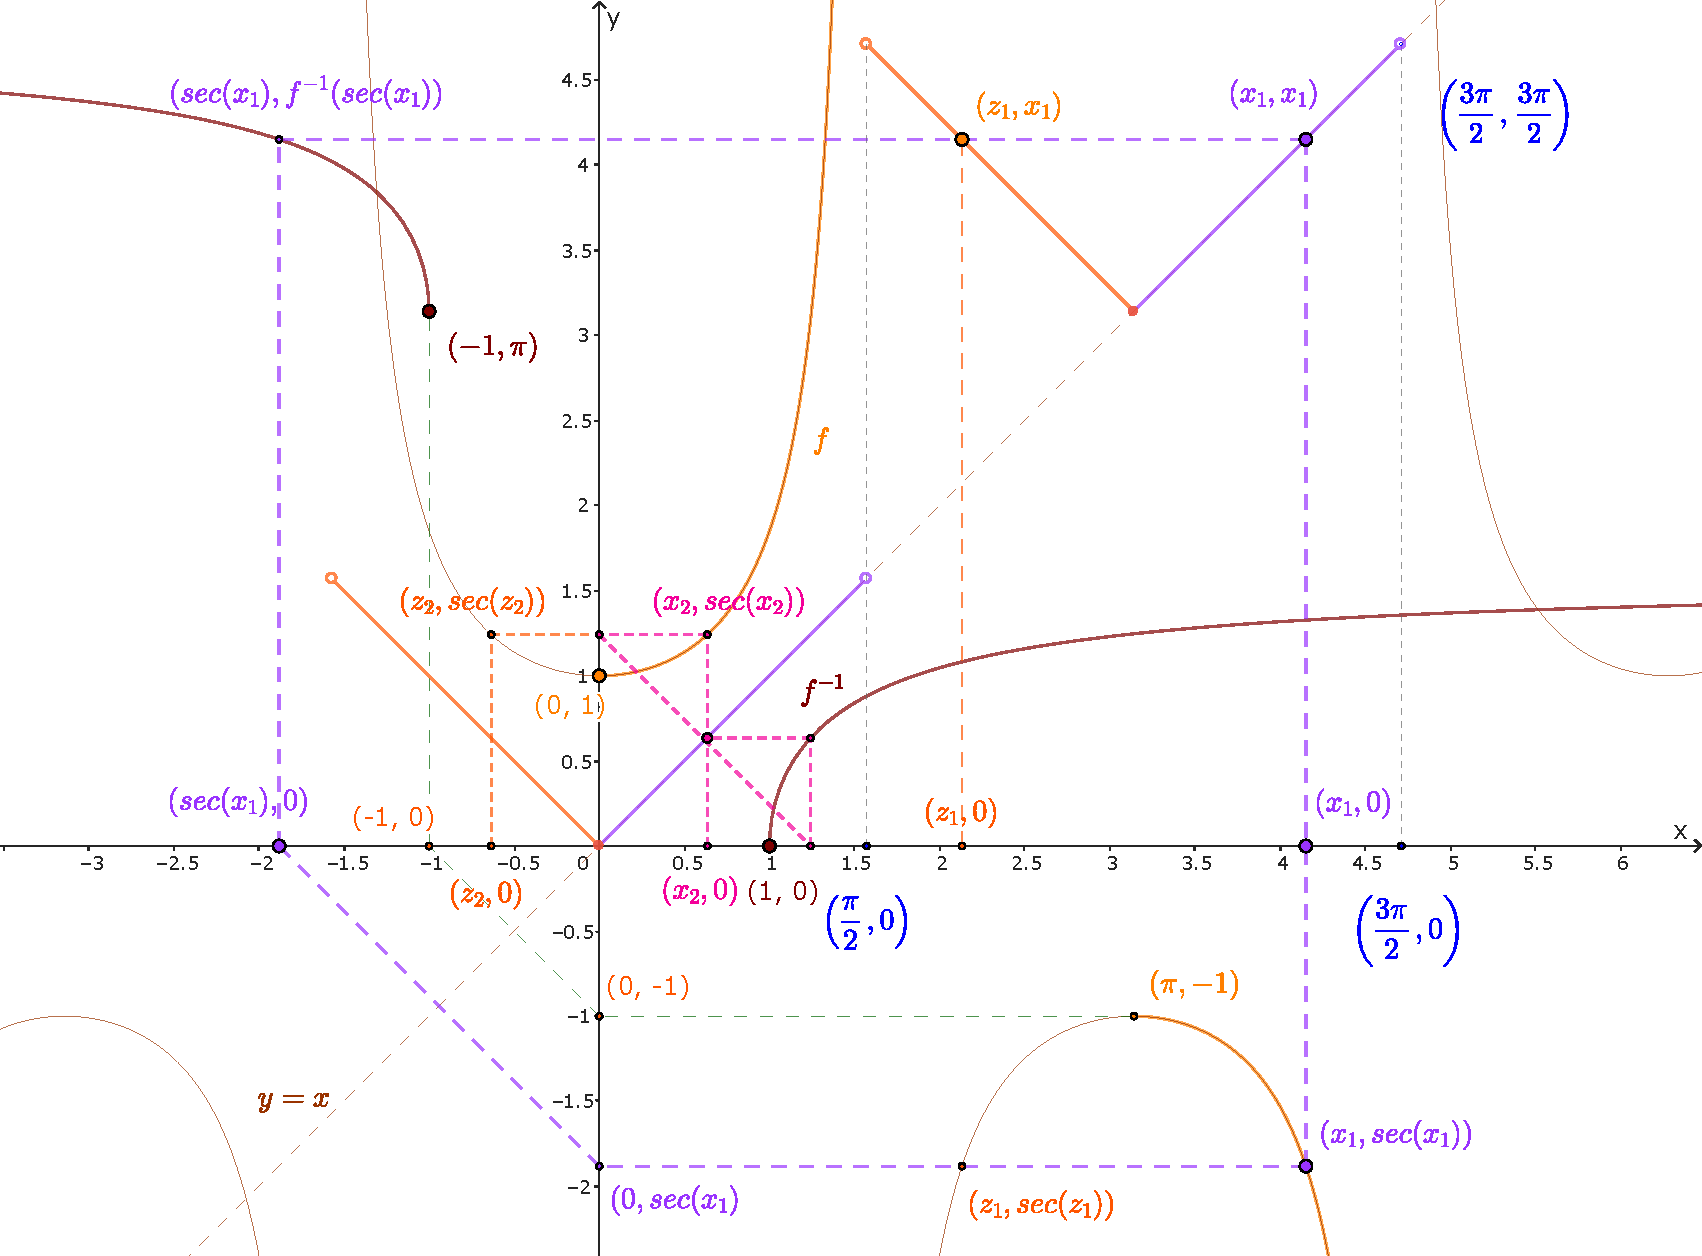
\includegraphics[width=16cm]{./svg/pdf/derivative-2-1d.pdf}
\end{center}

\begin{soln}
    Note that the graph of $\sec \circ f^{-1}$ consists of multiple functions
    \[
        (f^{-1} \circ \sec)(x) = 
        \begin{cases}
            -x + 2k\pi& \forall x \in \left( \frac{(4k-1) \pi}{2}, \frac{(4k) \pi}{2} \right]\\
            x - 2k\pi,& \forall x \in \left[ \frac{(4k) \pi}{2}, \frac{(4k+1) \pi}{2} \right)\\
            -x + 2(k+1)\pi,& \forall x \in \left( \frac{(4k+1) \pi}{2}, \frac{(4k + 2) \pi}{2} \right]\\
            x - 2k\pi,& \forall x \in \left[ \frac{(4k + 2) \pi}{2}, \frac{(4k+3) \pi}{2} \right)
        \end{cases}
    \]
\end{soln}

\newpage

\begin{problem*}[1e]
    Find a formula for the derivative of $f^{-1}.$
\end{problem*}

\begin{soln}
    Now let
    \[
        y = f^{-1}(x) = \sec^{-1}(x) \Rightarrow \sec(y) = x.
    \]

    Note that
    \[
        \begin{aligned}
            &\frac{d}{dx} \sec(x) = \frac{d}{dx} \frac{1}{\cos{x}} = - \frac{1}{(\cos{x})^2} \cdot \frac{d}{dx} \cos(x)
            = - \frac{1}{(\cos{x})^2} \cdot (- \sin{x}) =  \frac{1}{\cos{x}} \cdot \frac{\sin{x}}{\cos{x}} = \sec(x) \tan(x).\\
        \end{aligned}
    \]

    Differentiating both sides with respect to the variable $x,$
    \[
        \frac{d}{dx} \sec(y) = \frac{d}{dx} (x) 
        \Rightarrow \sec(y) \tan(y) \cdot \frac{dy}{dx} = 1
        \Rightarrow \frac{dy}{dx} = \frac{1}{\sec(y) \tan(y)}
    \]

    Note that from (1a),
    \[
        y \in R_{f^{-1}} = D_f = \left[ 0, \frac{\pi}{2} \right) \cup \left[ \pi, \frac{3\pi}{2} \right)
        \Rightarrow \cos{y}, \sin{y} \text{\ have same sign\ }
        \Rightarrow \tan(y) > 0.
    \]

    Note that $\sec(y) = x,$ hence
    \[
        \begin{aligned}
            &\tan^2(y) = \dfrac{\sin^2(y)}{\cos^2(y)} = 1- \dfrac{1}{\cos^2(y)} = 1 - \sec^2(y)\\
            &\Rightarrow \frac{dy}{dx} = \frac{1}{\sec(y) \tan(y)} = \frac{1}{\sec(y) \sqrt{1-\sec^2(y)}} = \boxed{\frac{1}{x \sqrt{1-x^2}}.}
        \end{aligned}
    \]
\end{soln}

\newpage

\begin{theorem*}[Mean Value Theorem]
    \label{theorem:mean-value-theorem}
    If $f$ is a continuous function on the closed interval $[a,b]$, with $a<b$, and $f$ is differentiable on $(a,b)$,
    then there exists some real number $c \in (a,b)$ such that 
    \[
        f'(c) = \frac{f(b)-f(a)}{b-a}.
    \]
\end{theorem*}

\begin{problem*}[2a]
    Let $a<b$ and $f$ be a function defined on $[a,b].$ Suppose that $f$ is a continuous function on $[a,b]$, and $f$ is differentiable on $(a,b)$, 

    Let $x \in \left[ a, b \right)$ and let $h > 0$ be such that $x+h \le b.$ Prove that there is $\theta \in (0,1)$ such that:
    \[
        \frac{f(x+h) - f(x)}{h} = f'(x+\theta h).
    \]
\end{problem*}

\begin{soln}
    First, note that $f$ is a continuous function on $[a,b]$, and $f$ is differentiable on $(a,b)$, and $[x, x+h] \subseteq [a,b],$
    thus $f$ is continuous on $[x, x+h]$ and $f$ is differentiable on $(x, x+h).$ 

    Second, by the \nameref{theorem:mean-value-theorem} for $f$ is continuous on $[x, x+h]$ and $f$ is differentiable on $(x, x+h),$ 
    there exists $c \in (x, x+h),$ such that:
    \[
        f'(c) = \frac{f(x+h)-f(x)}{(x+h) - x} = \frac{f(x+h) - f(x)}{h}.
    \]

    Now, by choosing 
    \[ 
        \theta = \dfrac{c-x}{h} \Rightarrow 0 = \dfrac{x-x}{h} < \theta = \dfrac{c-x}{h} < \dfrac{(x+h)-x}{h} = 1,\ x + \theta h = x + \dfrac{c-x}{h} \cdot h = c.
    \]        

    Hence, there exists $\theta \in (0,1)$ such that, 
    \[
        f'(x + \theta h) = f'(c) = \dfrac{f(x+h) - f(x)}{h}.
    \]
\end{soln}

\bigbreak

\begin{problem*}[2b]
    Consider $f(y) = \ln(y).$ Fix $x >0$ and $h>0.$ Find $\theta$ in term of $x$ and $h,$ as in the previous formula.
\end{problem*}

\begin{soln}
    First, it is easy to verify that $f=\ln$ is a continuous function on $[x,x+h]$, and is differentiable on $(x, x+h),$
    thus the conditions of the previous question apply.
    
    Now let $\theta$ be such that
    \[
        \begin{aligned}
            &(\ln(x + \theta h))' = \frac{\ln(x+h) - \ln(x)}{h} \Rightarrow \frac{1}{x + \theta h} = \frac{\ln(x+h) - \ln(x)}{h}\\
            &\Rightarrow x + \theta h = \frac{h}{\ln(x+h) - \ln(x)} \Rightarrow \theta = \boxed{\frac{h - x \ln(x+h) + x \ln(x)}{h(\ln(x+h) - \ln(x))}.}
        \end{aligned}
    \]
\end{soln}

\newpage

\begin{problem*}[2c]
    Fix $x >0.$ Find
    \[
        \lim_{h \rightarrow 0} \theta(x,h)
    \]
\end{problem*}

\begin{soln}[Solution 1]
    From the result from (2b),
    \[
        \theta = \frac{h - x \ln(x+h) + x \ln(x)}{h(\ln(x+h) - \ln(x))} = \frac{ h - x \ln(x+h) + x \ln(x) }{h^2} \cdot \frac{h}{\ln(x+h) - \ln(x)}
    \]

    By L'Hopital rule,
    \[
        \lim_{h \rightarrow 0} \frac{ h - x \ln(x+h) + x \ln(x) }{h^2} = \lim_{h \rightarrow 0 } \frac{\frac{d}{dh} (h - x \ln(x+h) + x \ln(x))}{\frac{d}{dh} h^2}
        = \lim_{h \rightarrow 0 } \frac{1 - \frac{x}{x+h}}{2h} = \lim_{h \rightarrow 0 } \frac{1}{2(x+h)} = \frac{1}{2x}.
    \]

    On the other hand,
    \[
        \lim_{h \rightarrow 0} \frac{h}{\ln(x+h) - \ln(x)} = \frac{1}{(\ln (x))'} = x.
    \]

    Thus,
    \[
        \lim_{h \rightarrow 0} \theta(x,h) = \frac{1}{2x} \cdot x = \boxed{\frac{1}{2}}
    \]
\end{soln}

\begin{soln}[Solution 2]
    Consider the generic case \textbf{with the assumption that the second derivative $f''$ exists} (which is obvious for (2b) since $f''(x) = -\frac{1}{x^2}$)
    \[
        \frac{f(x+h) - f(x) - hf'(x)}{h^2} = \frac{f'(x + \theta h) - f(x)}{h}  = \theta \cdot \frac{f'(x + \theta h) - f'(x)}{\theta h}
    \]

    By L'Hopital rule,
    \[
        \left\{
            \begin{aligned}
                &\lim_{h \rightarrow 0} \frac{f(x+h) - f(x) - hf'(x)}{h^2} = \lim_{h \rightarrow 0} \frac{f'(x+h)-f'(x)}{2h} = \frac{1}{2} f''(x)\\
                &\lim_{h \rightarrow 0} \theta \cdot \frac{f'(x + \theta h) - f'(x)}{\theta h} = 
                \lim_{h \rightarrow 0} \theta \cdot \lim_{(\theta h) \rightarrow 0} \frac{f'(x + (\theta h)) - f'(x)}{(\theta h)} = 
                \lim_{h \rightarrow 0} \theta \cdot f''(x)\\
            \end{aligned}
        \right.
    \]

    Thus $\theta = \boxed{\frac{1}{2}.}$
\end{soln}

\newpage

\begin{theorem*}[Intermediate Value Theorem]
    \label{theorem:intermediate-value-theorem}
    If $f$ is a continuous, real-valued function defined on an interval $[a,b]$, with $f(a) \not= f(b)$,
    and $y$ is a real number between $f(a)$ and $f(b)$, then there exists some $c \in (a,b)$ such that $f(c) = y$.
\end{theorem*}

\begin{problem*}[3a]
    Suppose that $f$ is continuous on $[a,b]$ and that $a < f(x) < b$ for all $x \in [a,b].$
    Prove that there exists $c \in (a, b)$ such that $c = f(c).$ 
    \textit{Hint: Consider the function $g(x) = x - f (x).$}
\end{problem*}

\begin{soln}
    Consider $g(x) = x - f(x),$ then $g$ is continuous on $(a,b),$ $g(a) = a - f(a) < 0$ and $g(b) = b - f(b) > 0.$
    By \nameref{theorem:intermediate-value-theorem}, there exits $c \in (a,b)$ such that $g(c) = 0,$ or $\boxed{c = f(c).}$
\end{soln}

\bigbreak

\begin{problem*}[3b]
    Suppose, in addition, that $f$ is differentiable on $(a,b)$ and that $|f'(x)| < 1$ for all $x \in (a,b).$
    Prove that there is a unique point $c \in (a, b)$ such that $c = f(c).$
    \textit{Hint: Use MVT.}
\end{problem*}

\begin{soln}
    From (3a) there exists a $c$ such that $c = f(c).$ We prove that it is unique.
    Assume the contrary, then exists $c_1 \ne c,$ $c_1 = f(c_1).$ WLOG, let $c < c_1.$

    By \nameref{theorem:mean-value-theorem} for then interval $(c, c_1),$ then there exists some real number $d \in (c,c_1)$ such that 
    \[
        f'(d) = \frac{f(c_1) - f(c)}{c_1 - c} = 1, \text{\ a contradiction since\ } |f'(x)| < 1,\ \forall x \in (c, c_1).
    \]
    
    Hence, $c$ is unique.
\end{soln}

\newpage

\begin{problem*}[3c]
    Using parts (a) and (b), show that the equation $\tan(3x) = \sqrt{2x + 1}$ has a unique solution on $(0, 1).$
    \textit{Formulate this equation as $x = f(x)$ for some function $f(x).$ Then use the results from part (a) and part (b)}
\end{problem*}

\begin{center}
    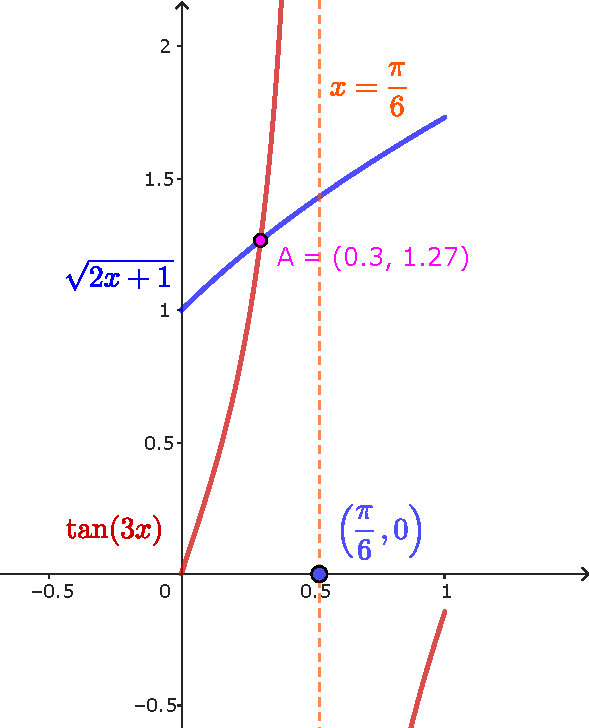
\includegraphics[width=7cm]{./svg/pdf/derivative-2-3c.pdf}
\end{center}

\begin{soln}
    First, note that :
    \begin{itemize}[topsep=0pt, partopsep=0pt, itemsep=0pt]
        \ii The function $\tan(3x)$ is strictly increasing from $0$ to $+\infty$ on $\left[ 0, \frac{\pi}{6} \right),$
        and stricly increasing from $-\infty$ to $\tan(1) \approx -0.142 < 0$ on $\left( \frac{\pi}{6}, 1 \right].$
        \ii On the other hand the function $\sqrt{2x + 1}$ is strictly increasing from $1$ to $\sqrt{3}$ on the whole interval $[0,1].$
    \end{itemize}

    Therefore $\sqrt{2x + 1} > \tan(3x),\ \forall x \in \left( \frac{\pi}{6}, 1\right].$

    Thus we shall only consider to find the unique solution only on the interval $I = \left[ 0, \frac{\pi}{6} \right).$
    Let
    \[
        f(x) = \tan(3x) - \sqrt{2x + 1}.
    \]
    
    Then $f$ is continuous on $I$ and $-1 \le f(x) < +\infty,\ \forall x \in I,$
    by \nameref{theorem:intermediate-value-theorem} $\exists c \in I: f(c) = 0.$

    If there exists $c_1 \ne c,$ $0 = f(c_1),$ then by \nameref{theorem:mean-value-theorem} for then interval $(c, c_1),$
    there exists some real number $d \in (c,c_1)$ such that 
    \[
        f'(d) = \frac{f(c_1) - f(c)}{c_1 - c} = 0 \quad (*)
    \]
    
    Note that
    \[
        f'(x) = \dfrac{3}{\cos^2(3x)} - \dfrac{1}{\sqrt{2x + 1}}, \text{\ and since\ } 3\sqrt{2x + 1} > 3 > \cos^2(3x) \Rightarrow f'(x) > 0,\ \forall x\in I.
    \]

    Thus (*) is a contradiction. Hence $c$ is unique.
\end{soln}

\newpage

\begin{problem*}[4]
    We are filling water from a conic tank (with vertex down) to a cylindrical tank.
    The conic tank has height 18 m and the radius of the base 6 m. The diameter of the cylindrical tank’s base is 10 m.
    We know the water level in the conic tank is decreasing at 1m/s when the water level is 12 m.
    Find the rate of change of the water level in the cylindrical tank.
\end{problem*}

\begin{soln}
    First, let calculate the volume of the conic tank. It is a (inverted) cone with base radius $r_1 = 6,$ height $h_1 = 18.$
    Therefore its \textit{full} volume is:
    \[
        V_1 = \frac{1}{3} \pi r_1^2 h_1,\text{\ where\ } r_1 : h_1 = 1 : 3.
    \] 

    If we consider $t$ as the variable of time, then $h$ is a function of $t,$ and $r$ can simply be calculated from $h$
    (the height and radius of the cone formed by the water are proportional to $h$ and $r$) 
    \[
        V_1(t) = \frac{1}{3} \pi r(t)^2 h(t) = \frac{\pi}{3} \left(\frac{1}{3} h(t) \right)^2 h(t) =  \frac{\pi}{27} h^3(t) \quad (*)
    \]

    When the water level is $12$ ($h(t) = 12$), the change in rate of the water level $h(t)$ in the conic tank is $-1,$ which means that $\dfrac{dh}{dt} = -1.$
    Thus the rate of change in water volume at the time $t$ ($h(t)=12$) is
    \[
        \frac{dV_1}{dt} = \frac{d}{dt} \left( \frac{\pi}{27} h^3(t) \right) = \frac{\pi}{9} h^2(t) \dfrac{dh}{dt} = \frac{\pi}{9} h^2(t) (-1)
        \Rightarrow \frac{dV_1}{dt} = - \frac{12^2 \pi}{9} = - 16\pi.
    \]

    This is the volume of water discharged from the conic tank into the cylindrical tank under it.
    The water volume that the cylindrical tank received must be the opposite of what the conic tank discharged:
    \[
        \frac{dV_2}{dt}(t) = - \frac{dV_1}{dt}(t) = 16\pi.
    \]

    The cylindrical tank volume function with radius $r_2 = \frac{10}{2}  = 5$ is $V_2(t) = \pi r_2^2 h(t),$ therefore:
    \[
        \frac{dV_2}{dt} = 25 \pi \frac{dh}{dt} \Rightarrow 16\pi = 25 \pi \frac{dh}{dt}  \rightarrow \frac{dh}{dt}  = \boxed{\frac{16}{25}} \text{\ m/s.}
    \]
\end{soln}

\newpage

\begin{problem*}[5]
    Let $0 < a < b < 2a.$ We will consider the curve $xy=1$ on $[a,b].$ We now sketch a tangent line at any point $(x,y)$ on this curve with $x-$coordinate in $[a,b].$
    Then we will have a trapezoid and its four sides are on this tangent line, $x-$axis, $x = a$ and $x = b.$
    Find the point $(x, y)$ such that the area of the trapezoid is the largest.
\end{problem*}

\begin{center}
    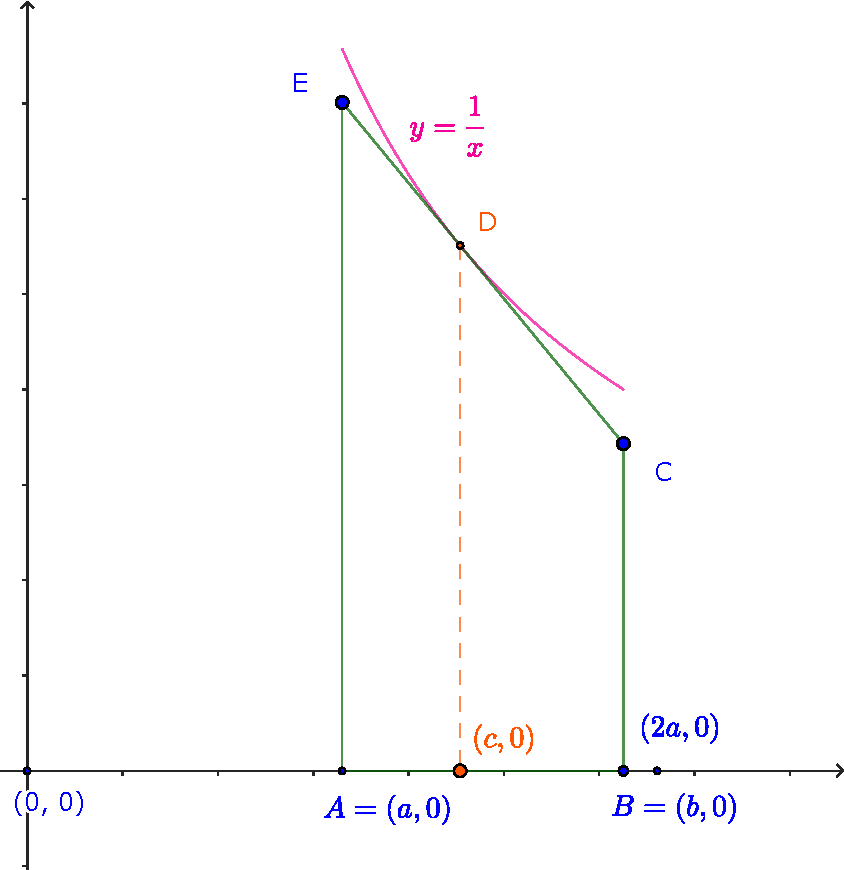
\includegraphics[width=10cm]{./svg/pdf/derivative-2-5.pdf}
\end{center}

\begin{soln}
    Let $D \left(c, \frac{1}{c} \right)$ the point. Then 
    \[
        a < c < b < 2a \Rightarrow a < c < b < 2a < 2c \quad (*)
    \]
    
    The slope of the tangent line is $f'(c) = -\dfrac{1}{c^2},$ thus the equation of the tangent line through $D$ is:
    \[
        y -  \frac{1}{c} = \left( -\frac{1}{c^2} \right) (x-c) \quad (*)
    \]

    Thus $C$ and $E$ coordinates are
    \[
        C \left( b, -\frac{1}{c^2}(b-c) + \frac{1}{c} \right) \text{\ or\ } C\left( b, \frac{2c - b}{c^2} \right),\ 
        E \left( a, -\frac{1}{c^2}(a-c) + \frac{1}{c} \right) \text{\ or\ } E\left( a, \frac{2c - a}{c^2} \right).
    \]

    The distances $BC$ and $AE$:
    \[
        BC = \frac{2c - b}{c^2},\ AE = \frac{2c - a}{c^2}
        \Rightarrow \half(BC + AE) = \half \left( \frac{2c - b}{c^2} + \frac{2c - a}{c^2} \right) = \frac{4c - a - b}{2c^2}
    \]

    Thus the area $[ABCE],$
    \[
        [ABCE] = AB \cdot \half(BC + AE) = (b-a)\frac{4c - a - b}{2c^2}
    \]

    Now, let 
    \[
        f(c) = \frac{4c - a - b}{2c^2} = \frac{2}{c} - \frac{a+b}{2c^2} 
        \Rightarrow \frac{df}{dc} = -\frac{2}{c^2} + \frac{a+b}{c^3} = \frac{1}{c^2}(a+b-2c) \quad(*)
    \]

    Note that if $\dfrac{1}{c^2}(a+b-2c)$ is positive if $c < \half(a+b),$ and negative otherwise.
    Thus $f$ increase from $c = a$ until $c= \half(a+b)$, then $f$ decreases from $c= \half(a+b)$ until $c=b.$
    Therefore 
    \[
        f_{max} = f\left(\frac{a+b}{2}\right) = \frac{2(a+b) - a - b}{\half(a+b)^2} = \boxed{\frac{2}{a+b}.}
    \]

    \textit{Note: We can also give a direct proof for the upper limit, and then show that $f\left(\frac{a+b}{2}\right)$ is equal to this limit;}
    \[
        \frac{4c - a - b}{2c^2}  \le \frac{2}{a+b} \Leftrightarrow 4c(a+b) - (a+b)^2 \le 4c^2 \Leftrightarrow (2c -a -b)^2 \ge 0.
    \]
\end{soln}


\end{document}